\section{Data, Labels and the Narrative Landscape (RQ1)}
\label{sec:data}

\begin{figure}[t]
  \centering
  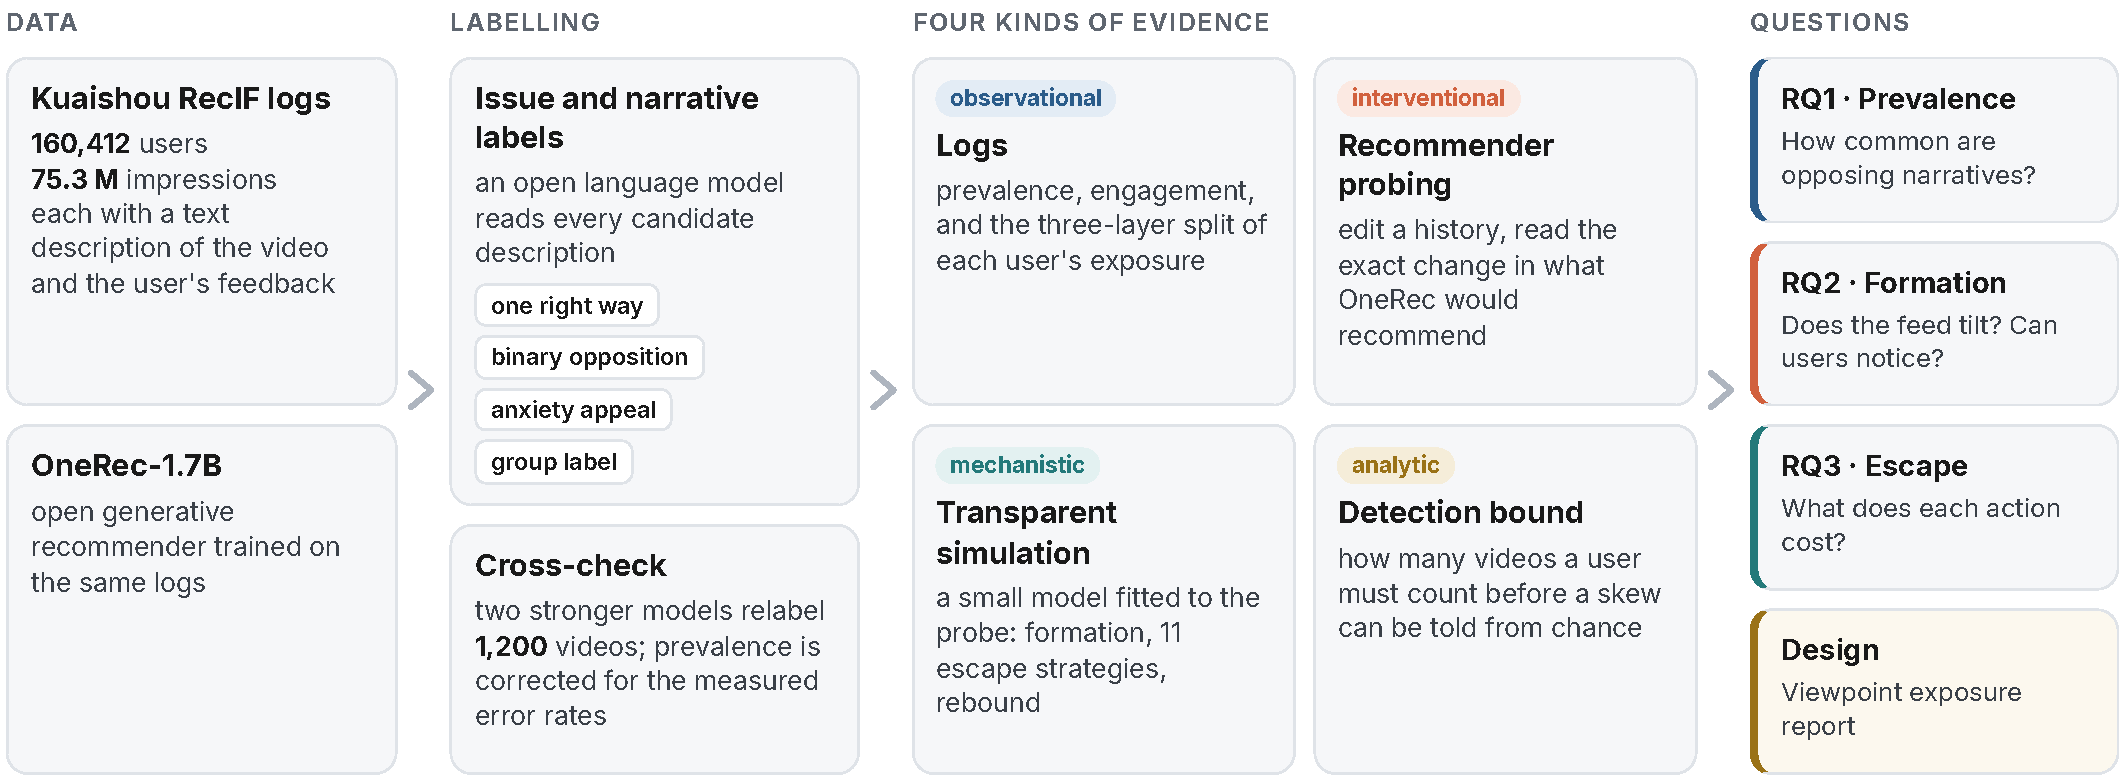
\includegraphics[width=\textwidth]{figures/fig_overview.pdf}
  \caption{Study design. Language-model labels turn the logs into exposure counts for issues and narratives. Four kinds of evidence, each with a different strength, are then combined: the logs describe what users were shown, probing shows how the recommender responds to a controlled change, the simulation follows the consequences over months, and a statistical bound says what a user could notice.}
  \label{fig:overview}
\end{figure}

\subsection{Data}

\Cref{fig:overview} summarises the design. RecIF is the public interaction log released with the OpenOneRec project~\citep{zhou2025openonerec}. Our extract holds 160{,}412 users and 75.3 million impressions. Each impression records the video, a text description of its content, and the user's feedback: whether the video was watched to the end, liked, commented on, shared, or marked ``not interested''. We never see the videos themselves. OneRec-1.7B, released by the same project, is a generative recommender trained on these logs: it reads a user's history as a sequence of semantic video IDs, grouped by feedback type, and generates the IDs of videos to recommend. Because its vocabulary is closed, the probability it assigns to any candidate video can be computed exactly.

We chose logs with an open recommender over the two alternatives. Scripted accounts on the live app~\citep{haroon2023youtube,kaplan2026foryou} observe the production system, but cannot separate supply from ranking, are limited to a few hundred accounts, and manipulate a live service. A purely synthetic simulation~\citep{chaney2018confounding,jiang2019degenerate} is transparent but its responses are assumed. Logs give exposure for a whole population, and the open model lets us measure the response to a user action instead of assuming it.

\subsection{Labelling pipeline}

\paragraph{Taxonomy.} We first read 500 uniformly sampled impressions and grouped the social issues that recur into five domains (\cref{tab:landscape}). Politically sensitive issues are excluded: labels for them are contested, and they are hard to discuss openly. Across domains, four types of opposing narrative recur (\cref{tab:taxonomy}). The case study uses the sharpest of them in the largest domain: a \emph{gender group label} is a video that (i) targets a whole gender, not a person, (ii) attributes a negative trait or blame, (iii) generalises it to all or most members, and (iv) asserts it in its own voice. A video that quotes such a claim in order to rebut it is a \emph{rebuttal} and belongs to the retained set.

\begin{table}[t]
\caption{The four types of opposing narrative. Examples are paraphrased from video descriptions in the gender-and-marriage domain.}
\label{tab:taxonomy}
\centering\small
\begin{tabularx}{\textwidth}{@{}L{2.5cm} L{5.4cm} Y@{}}
\toprule
Type & Definition & Example\\
\midrule
One right way & presents one choice as the only acceptable one & ``Not married by thirty? Then you have already lost.''\\
Binary opposition & reduces the issue to two camps with nothing between & ``Marry for love or marry for money. There is no third kind of marriage.''\\
Anxiety appeal & argues through the threat of loss or failure & ``Wait two more years and nobody will want you.''\\
Group label & attaches a negative trait to a whole group of people & ``Women today only look at the bride price.'' ``Men all stop trying once the wedding is over.''\\
\bottomrule
\end{tabularx}
\end{table}

\paragraph{Labels.} A recall-oriented screen, made of keywords and of embedding similarity to seed descriptions, selects 684{,}210 candidate videos (5.9 million impressions). An open model run locally, Qwen3-30B, then reads each description and answers a fixed sequence of questions: which domain, if any; whether the video carries an opposing narrative and of which type; and the four questions of the group-label rule (prompt in \cref{app:prompt}). Of the candidates, 212{,}480 are labelled as gender-and-marriage videos; these form the case-study corpus, with 1.77 million impressions.

\paragraph{Quality.} No video was labelled by hand, so label quality is established by agreement with stronger models. Two reference models, DeepSeek V4 Pro and GPT-6.1 Sol, independently relabelled 1{,}200 videos, sampled in proportion to exposure and enriched with videos the open model had flagged. Where the two agree (93\% of decisions) their label is the reference; the rest are settled by a third pass with the full guideline. \Cref{tab:quality} reports Cohen's $\kappa$~\citep{cohen1960kappa}. Agreement is substantial or better on the scale of \citet{landis1977agreement} for every decision except the four-way type, which we therefore use only in aggregate. For the group-label decision the open model has recall $\alpha=0.79$ and false-positive rate $\beta=0.010$. All prevalence figures below are corrected for these rates~\citep{rogan1978prevalence}, and the same two numbers describe the classifier a user-side tool could realistically run (\cref{sec:detection}).

\begin{table}[t]
\caption{Label quality on 1{,}200 validation videos. $\kappa$ is Cohen's kappa; precision and recall are those of the open model against the reference label.}
\label{tab:quality}
\centering\small
\begin{tabular}{@{}lcccc@{}}
\toprule
Decision & $\kappa$ (open vs.\ reference) & $\kappa$ (between references) & Precision & Recall\\
\midrule
On one of the five issues & 0.81 & 0.88 & 0.90 & 0.87\\
Opposing narrative (yes/no) & 0.74 & 0.82 & 0.81 & 0.83\\
Narrative type (four-way) & 0.69 & 0.78 & -- & --\\
Gender group label (yes/no) & 0.78 & 0.86 & 0.84 & 0.79\\
\bottomrule
\end{tabular}
\end{table}

\subsection{Results: how common, which types, how engaging}

To estimate prevalence without relying on the screen, we drew 20{,}000 impressions uniformly from all users' histories, so that a video counts in proportion to how often it was shown, and labelled them with the reference models.

\paragraph{About one impression in thirteen is on a social issue, and almost a fifth of those take a side.} The five domains account for \nIssueShare\% of impressions (\cref{tab:landscape}, \cref{fig:landscape}a). Of these issue impressions, \nOppShare\% (95\% CI \nOppShareLo--\nOppShareHi) carry an opposing narrative. The share is highest for gender and marriage (24\%) and body and appearance (21\%), and lowest for family matters (9\%).

\paragraph{Each domain has its own way of taking sides.} Body-and-appearance videos argue mostly through anxiety, life-choice videos through the one right way, and gender-and-marriage videos through binary oppositions and group labels (\cref{fig:landscape}b). Group labels are rare outside gender and marriage, where they make up 6.2\% of impressions.

\paragraph{Opposing narratives are engaging, and ranking shows more of them than supply contains.} Compared with other issue videos of the same domain and length, an opposing narrative is more likely to be finished (odds ratio 1.19), liked (1.22) and shared (1.33), and far more likely to be commented on (1.85; \cref{fig:landscape}c). Group labels draw the most comments of all (2.41). They are also marked ``not interested'' 2.4 times as often, so the engagement they attract is not approval; this matches the finding that engagement-based ranking amplifies divisive content that users do not say they want~\citep{milli2025engagement}. In every domain the exposure share of opposing narratives exceeds their share among distinct videos, by a factor of 1.2 to 1.5 in odds (last column of \cref{tab:landscape}). This is the platform layer of \cref{eq:decomp}, and it is present before any personalisation.

\begin{table}[t]
\caption{Social issues and opposing narratives in a uniform sample of 20{,}000 impressions. ``Opposing'' is the share of the domain's impressions that carry an opposing narrative (95\% Wilson interval). ``Amplification'' is the odds of an opposing narrative among impressions divided by its odds among distinct videos, computed on the issue corpus.}
\label{tab:landscape}
\centering\small
\setlength{\tabcolsep}{5pt}
\begin{tabular}{@{}lrrlrrrrr@{}}
\toprule
 & \multicolumn{2}{c}{Impressions} & & \multicolumn{4}{c}{Opposing narratives by type} & \\
\cmidrule(lr){2-3}\cmidrule(lr){5-8}
Domain & $n$ & \% of all & Opposing, \% & \makecell[r]{One\\right way} & \makecell[r]{Binary\\oppos.} & \makecell[r]{Anxiety\\appeal} & \makecell[r]{Group\\label} & \makecell[r]{Amplifi-\\cation}\\
\midrule
\tabinput{generated/tab_landscape_body}
\bottomrule
\end{tabular}
\end{table}

\begin{figure}[t]
  \centering
  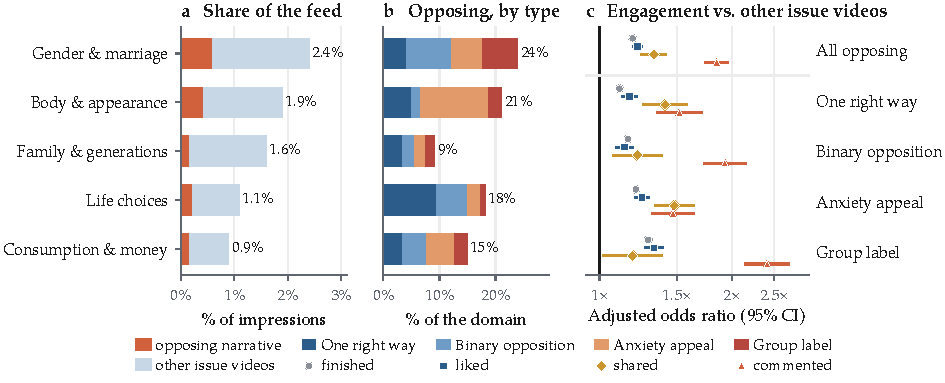
\includegraphics[width=\textwidth]{figures/fig_landscape.pdf}
  \caption{The narrative landscape. \textbf{(a)} Share of all impressions taken by each domain, with the part that carries an opposing narrative. \textbf{(b)} Opposing narratives as a share of each domain's impressions, by type. \textbf{(c)} Odds ratios of four kinds of engagement for opposing narratives against other issue videos, from logistic regressions on 5.9 million issue impressions with domain and video-length controls and standard errors clustered by user.}
  \label{fig:landscape}
\end{figure}
